% !TEX root = ../thesis.tex
%
\chapter{Preliminary Studies}
\label{sec:preliminary}

In order to determine the usability of Ohua for implementing shared state applications and to identify any necessary modifications to the compiler or the runtime, we first tried to implement a single such application with it.
After successful implementation we wanted to compare its performance against a Software Transactional Memory implementation of the same program and see, whether there are any shortcomings of Ohua in terms of performance.
Based on this initial study we then wanted to find ways to improve Ohua's performance, if necessary, e.g., by introducing new compiler optimizations.
The aim of these preliminary studies was to find out, whether Ohua was usable for writing programs relying on shared state and if it could be a viable alternative to STM in this setting.

\section{Labyrinth Benchmark}

As a first example application, we chose to implement the \emph{labyrinth} benchmark as presented by Swalens et al.~\cite{swalens2016transactional}.
This algorithm is a variation of Lee's Algorithm~\cite{lee1961algorithm} which solves path-connection problems often encountered when searching for an optimal route or generating wiring diagrams where wires may not overlap.
We base our own implementation on the descriptions of Watson et al.~\cite{watson2007study}, who presented an implementation for Transactional Memory.

\begin{figure}[b]
    \begin{subfigure}[t]{.24\textwidth}
        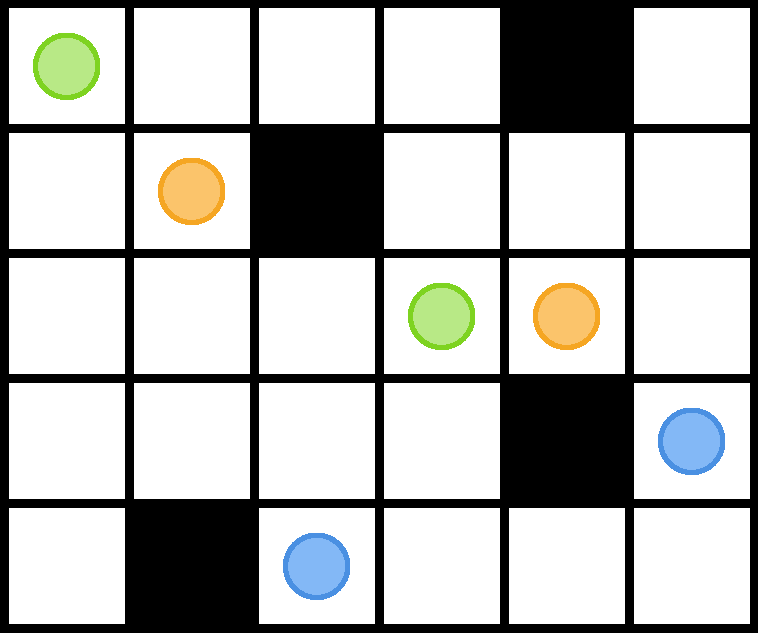
\includegraphics[width=\textwidth,keepaspectratio]{gfx/preliminaries-labyrinth/1-maze_points}
        \caption{Initial grid with 3 point pairs.}%
    \end{subfigure}%
    ~
    \begin{subfigure}[t]{.24\textwidth}
        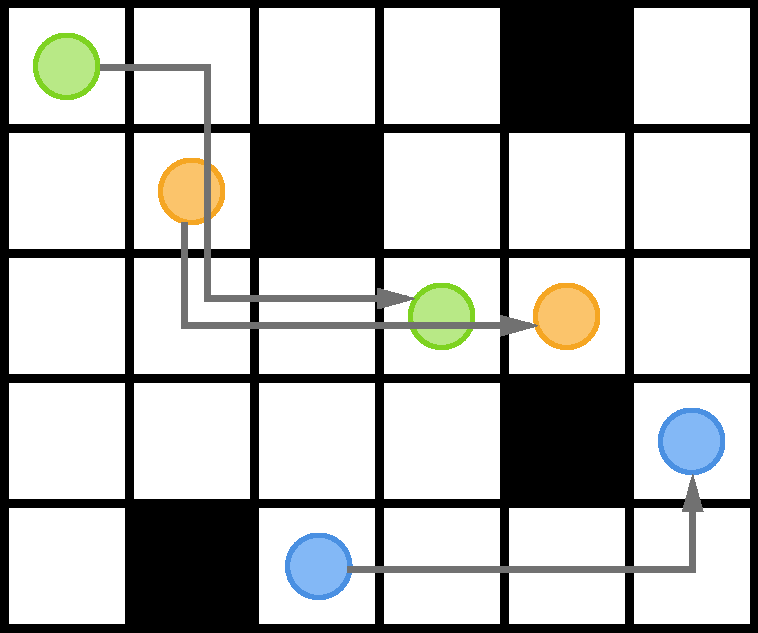
\includegraphics[width=\textwidth,keepaspectratio]{gfx/preliminaries-labyrinth/2-maze_paths}
        \caption{Possible paths between the points.}%
    \end{subfigure}%
    ~
    \begin{subfigure}[t]{.24\textwidth}
        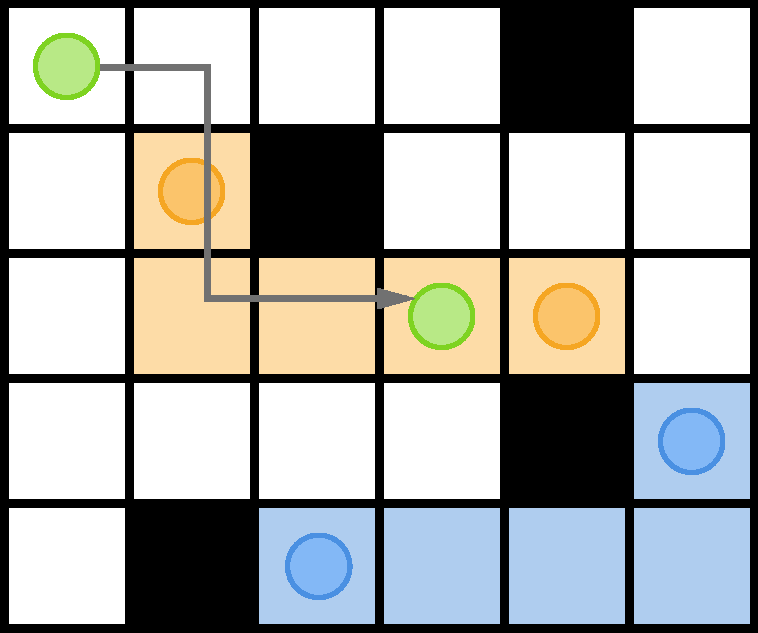
\includegraphics[width=\textwidth,keepaspectratio]{gfx/preliminaries-labyrinth/4-maze_update2}
        \caption{First two paths are mapped into the maze.}%
    \end{subfigure}%
    ~
    \begin{subfigure}[t]{.24\textwidth}
        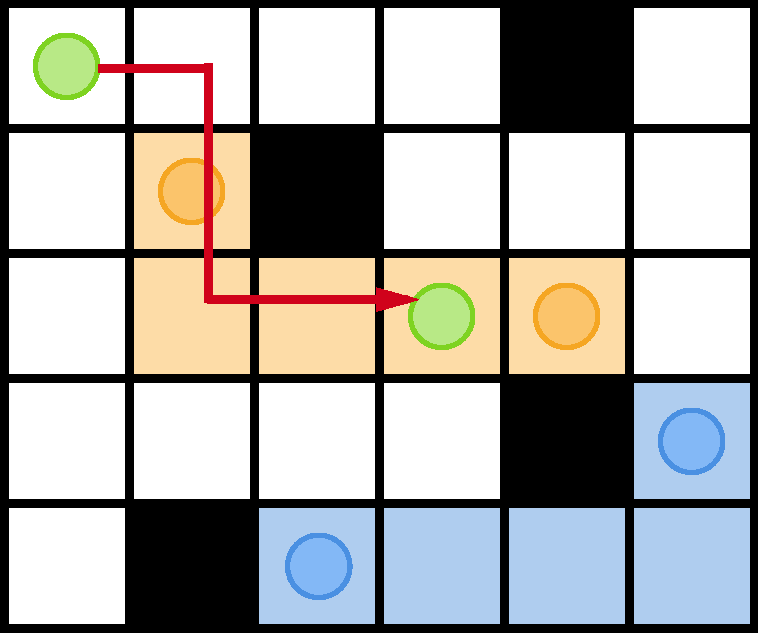
\includegraphics[width=\textwidth,keepaspectratio]{gfx/preliminaries-labyrinth/5-maze_update3}
        \caption{Conflict for the third path as it goes through a now-occupied segment.}%
        \label{fig:preliminary:labyrinth:unroutable}
    \end{subfigure}%
    \caption{Illustration of the operation of the labyrinth benchmark, showing the (attempted) mapping of 3 paths in a 6 $\times$ 5 two-dimensional grid. Black squares represent walls that cannot be routed through.}%
    \label{fig:preliminary:labyrinth}
\end{figure}

Goal of the benchmark is to find a number of paths within a three-dimensional maze, as depicted in Fig.~\ref{fig:preliminary:labyrinth}.
As input, the algorithm is provided with a maze and a set of pairs of points, between which a path is to be found and mapped within the maze.
During execution, one pair of coordinates is removed from the list of points (the worklist) and the program attempts to find a path between both points in the maze.
This is done using a breadth-first search.
The maze itself may also contain \enquote{walls} (highlighted as black squares in Fig.~\ref{fig:preliminary:labyrinth}), through which no path can be routed.
Also, each point in the maze may only be occupied by a single path to rule out overlapping paths.
The algorithm terminates once the worklist is empty and all paths have either been mapped successfully or deemed unmappable by the absence of a valid connection between both points.

This benchmark is a classic example for an \emph{irregular application}: all operations happen on the shared maze data structure which is modified in the process.
Additionally, any data parallelism obtainable in the application is \emph{amorphous}, as mapping one path in the maze may render another pair of coordinates unroutable as both points get cut off from one another.
An example for this can be seen in Fig.~\ref{fig:preliminary:labyrinth:unroutable}, where the mapping of the orange path makes finding a path between the green coordinates impossible as one point is part of the orange path.
As we have learned in chapter~\ref{sec:background:irregular}, this specific class of problems can be parallelized easily using Software Transactional Memory.
Searching for a single path can be compartmented into a transaction, treating all maze fields as transaction variables.
Listing~\ref{fig:preliminaries:stm} shows the resulting transactional implementation of the labyrinth benchmark.

\begin{listing}[t]
    \begin{minted}[fontsize=\footnotesize]{Rust}
        let (worklist, grid) = /* read from file */

        for points in worklist {
            atomically(|trans| {
                let local_grid = create_working_copy(&grid);

                if let Some(path) = find_path(points, &local_grid) {
                    // if path is found, write back results
                    update_grid(&grid, &path, trans)?;
                }

                Ok(())
            });
        }
    \end{minted}
    \caption{Simple implementation of the labyrinth benchmarks using Software Transactional Memory in Rust.}%
    \label{fig:preliminaries:stm}
\end{listing}

All path pairs are collected in a worklist, through which the algorithm iterates (line 3).
Inside the transaction that is started for each item (line 4), a working copy of the maze is created as detailed in~\cite{swalens2016transactional} to reduce the number of repeated reads from individual transaction variables.
Then, the breadth-first search commences in order to discover a route between the starting point and the target (line 7).
Note that since we've made a copy of the grid beforehand, this happens completely locally.
When a path is found, an update is run on the grid, inserting the path (line 9).
Should another transaction, which also happened to alter one or more segments of the newly-found path, manage to commit in the meantime, the resulting conflict is detected and the transaction is rolled back and re-run until either the update commits successfully or no path can be found anymore.
Our transactional memory implementation is a mere adaption of the algorithm outlined above, augmented with concurrency by splitting the worklist into $n$ parts, which are processed by $n$ threads in parallel.

In our first Ohua implementation, we described idiomatically, what the algorithm should be doing.
Listing~\ref{fig:preliminaries:ohua1} shows this simple program: First, all paths are searched for individually (lines 2-4), before they are written to the grid (line 6).
If a path conflicts with a previously saved one (i.e., at least one segment of the path is not free anymore), it is scheduled for re-computation by adding it to the \rust{remap_paths} vector.
Until all paths have either been mapped or discarded as unroutable, these steps are repeated recursively, although this invocation has been omitted from the sample code for the sake of simplicity.

\begin{listing}[t]
    \begin{minted}[fontsize=\footnotesize]{Rust}
        fn fill(maze: Maze, to_map: Vec<(Point, Point)>) -> Maze {
            let paths = for pair in to_map {
                find_path(maze, pair)
            };

            let (remap_paths, new_maze) = update_maze(maze, paths);

            // recursively call `fill` as necessary
        }
    \end{minted}
    \caption{Simplified first implementation of an recursive Ohua algorithm for the labyrinth benchmark}%
    \label{fig:preliminaries:ohua1}
\end{listing}

This implementation resembles an executable version of an Ohua algorithm that did compile and run with the initial Ohua compiler framework.\todo{Clarify distinction between Ohua versions: Which is default?}
In contrast to the STM algorithm, the maze update has been moved out of the inner loop, since this operation should remain sequential, following Ohua's idea of fostering local state, as introduced in chapter~\ref{fig:background:ohua}.

% TODO: Maybe subsection?
\subsection{First Results}

To establish a baseline for performance comparison, we measured the execution time of both benchmarks and calculated the speedup in relation to a sequential implementation, as outlined in chapter~\ref{sec:experiments:measurements}.
In an attempt to achieve comparable results, we used the same input data that had also been used previously by other authors and was originally proposed by Minh et al.~\cite{minh2008stamp}.
The chosen input maze for our test run had a size of 128 $\times$ 128 $\times$ 5 cells and required the mapping of 128 paths, given as predefined coordinate pairs, into it.
Resulting speedup figures for a varying number of worklist splits are shown in Fig.~\ref{fig:preliminaries:initial-results}.

\begin{figure}[h]
    \centering
    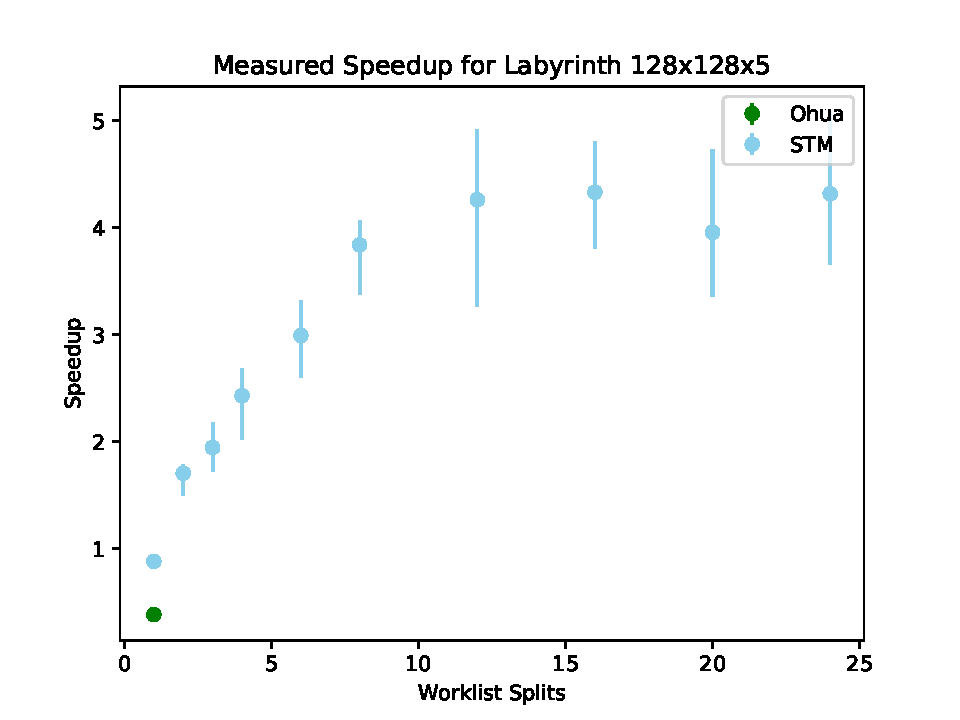
\includegraphics[width=.5\textwidth,keepaspectratio]{gfx/preliminaries-labyrinth/2019-04-18-128x128x5}
    \caption{Measured speedups of the labyrinth application for the STM and Ohua implementations.}%
    \label{fig:preliminaries:initial-results}
\end{figure}

As one can see in the plot, Software Transactional Memory is able to achieve a logistic growth for its speedup for 1 to 24 worklist splits, which converges at a mean maximum speedup of about 4.3.
Ohua on the other hand recorded only a single measuring point for a run with no worklist splitting at all.
This single run exhibited a speedup of less than 0.5, meaning it took more than twice as long to complete as the sequential reference implementation.
The reason for this is the absence of any configuration options for e.g. worklist splits.
Hence, there is no data parallelism in the Ohua algorithm, as the Rust runtime does not support parallel loops yet.
Effectively, this single measurement shows the performance of a sequential algorithm executed with the Ohua runtime, revealing the overhead it has compared to a normal sequential implementation.
Most of the overhead stems from the spawning of the threads each operator lives in and the resulting movement of data between these threads.\todo{Maybe produce a diagram showing the overhead in comparison?}
Our hope is to show that these overheads amortise with increased data parallelism.

In order to achieve more data parallelism and an overall improved performance, we were looking for modifications that could be made to the Ohua algorithm to accomplish this.
We first wanted to introduce manual changes to the algorithm without making amendments to the compiler to test different approaches easily.
These manual changes simply emulate the changes a compiler pass would make on the algorithm layer.
After identifying the optimizations that indeed provide a performance boost, we generalized them into compiler optimizations applicable to all algorithms.
The resulting transformations will be discussed in chapter~\ref{sec:transformations}.


\section{Parallel Loop Implementation}

As Fig.~\ref{fig:preliminaries:initial-results} clearly showed, the most pressing issue with the existing Ohua implementation for Rust was the absence of any data parallelism facilities like parallel loops.
Our first assumption based on these results was, that most performance could be gained simply by processing multiple labyrinth paths in parallel, as this operation makes up for most of the execution time in the sequential implementation.\todo{Show graphics that outline what takes how long. Take data from flamegraph}
The idea was to split the worklist into $n$ equally sized chunks and process them in parallel, which is similar to what STM does.
Listing~\ref{fig:preliminaries:ohua2} shows an exemplary implementation for an algorithm splitting the worklist in two parts.
Lines that were changed compared to the previous iteration are highlighted.

\begin{listing}[b]
    \begin{minted}[fontsize=\footnotesize,highlightlines={2-10}]{Rust}
        fn fill(maze: Maze, to_map: Vec<(Point, Point)>) -> Maze {
            let (tm0, tm1) = splitup(to_map);
            let part0 = for pair in tm0 {
                find_path(maze, pair)
            };
            let part1 = for pair in tm1 {
                find_path(maze, pair)
            };

            let paths = join(part0, part1);

            let (remap_paths, new_maze) = update_maze(maze, paths);

            // recursively call `fill` as necessary
        }
    \end{minted}
    \caption{Labyrinth implementation in Ohua using worklist splits for parallelism.}%
    \label{fig:preliminaries:ohua2}
\end{listing}

The main difference to the previous iteration of the algorithm is the introduction of two new operators, \rust{splitup} and \rust{join}.
These are implemented in the user space for this example but would become part of the runtime when this alteration is translated into a compiler transformation.
Their task is simply to split the worklist up into the required number of parts and merge them back together, once results have been produced.
Data parallelism is introduced in a very verbose manner by the duplication of the loop (lines 3-8).
This change can be scaled for an arbitrary number of threads by partitioning the worklist into as many parts as necessary for testing purposes.

% discuss the effect of this change (i.e., did it work? graph!)
Introducing a rudimentary form of data parallelism helped not only to obtain multiple meaningful measurements for Ohua, but also led to better performance, as can be seen in Fig.~\ref{fig:preliminaries:split-results}.
It now also exhibits a performance growth behavior that can roughly be described as logistic, though it only manages to achieve half as much speedup as STM.
Upon investigating this performance gap we determined two fundamental problems resulting from our current algorithm: Retries and Stragglers.

\begin{figure}[h]
    \centering
    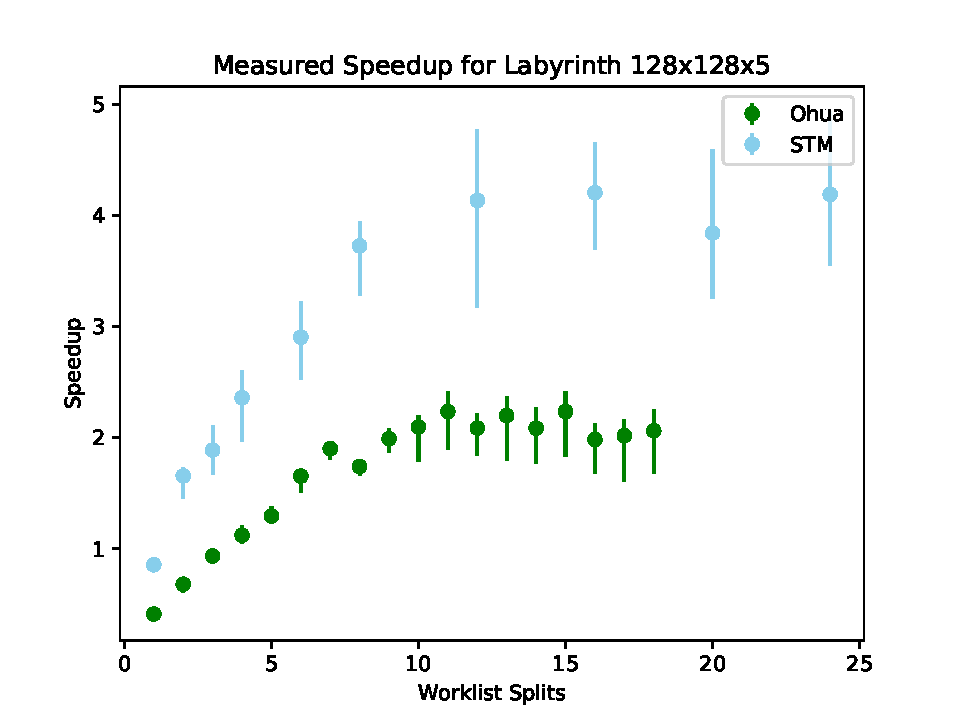
\includegraphics[width=.5\textwidth,keepaspectratio]{gfx/preliminaries-labyrinth/split_128x128x5}
    \caption{Measured speedup for an Ohua implementation using worklist splits.}%
    \label{fig:preliminaries:split-results}
\end{figure}

Besides data parallelism, another important factor influencing the execution time of the benchmark\footnote{In fact, this holds true for any irregular application following this \emph{Calculate-Update Pattern}.} is the number of repeated calculations that is necessary.
As described before, the labyrinth benchmark is designed to repeatedly attempt to find a route between each coordinate pair until a path is either successfully mapped or no valid path can be found anymore.
In the sequential implementation, this is not an issue as each path is searched for and updated individually without any concurrency, guaranteeing that each coordinate pair will only ever be evaluated once.
Any concurrent implementation however, comes at the cost of potential write conflicts that need to be resolved.
STM for example uses $n$ threads, always working on finding $n$ paths in parallel which are then written to the maze.
This means that from the perspective of one thread, in between its last access to the maze and an attempted update, about $n - 1$ changes will ideally have been made to the maze, each possibly introducing a conflict provoking a recomputation of the given path.
So at worst, per iteration of $n$ threads, $n-1$ results may become invalid due to a write conflict, forcing recomputation.\\
For Ohua, this number is significantly higher.
Its current approach is to update the shared state as late as possible, after computing all paths.
The negative side effect of this is that in a run to map $p$ paths, $p-1$ results may require a recomputation per recursion step in the worst case, possibly leading to as much as $\sum_{0 \leq i < p} i$ conflicts, which may in part explain the bad performance of Ohua.\todo{Maybe add some data about retries? (Numbers for Ohua and STM)}

The second relevant performance bottleneck is the straggler problem.
In research, when reasoning about parallel tasks it is often assumed that all tasks perform uniformly, i.e., require the same time to complete.
Real applications however rarely fulfill this assumption.
On the contrary, the tasks in these worklists are often wildly heterogeneous, each requiring a different amount of processing time.
This is also the case in the labyrinth benchmark.
The processing time for a single path depends solely on the number of nodes the path finder has to inspect which is related to the distance between the starting coordinates and the target.
As result, the $n$ threads of our algorithm each take differently long to process their worklist, which means that all threads finishing their work earlier have to wait at the synchronization point for all slower threads to finish.
This forced slack time is also present in the STM algorithm implementation, yet not as severe as in the Ohua implementation, since it synchronizes all threads only once when terminating them, while Ohua's threads synchronize once per recursion step.\todo{Maybe add a straggler graph?!}


\section{Lowering the Retry Count}
\label{sec:preliminaries:retries}

\begin{listing}[!b]
    \begin{minted}[fontsize=\footnotesize,highlightlines={2,14}]{Rust}
        fn fill(maze: Maze, to_map: Vec<(Point, Point)>, frequency: usize) -> Maze {
            let (points, still_to_map) = take_n(to_map, frequency);
            let (tm0, tm1) = splitup(points);
            let part0 = for pair in tm0 {
                find_path(maze, pair)
            };
            let part1 = for pair in tm1 {
                find_path(maze, pair)
            };
        
            let paths = join(part0, part1);
        
            let (remap_paths, new_maze) = update_maze(maze, paths);
            let to_remap = join(remap_paths, still_to_map);
        
            // recursively call `fill` as necessary
        }
    \end{minted}
    \caption{Ohua algorithm using a fixed update frequency to lower the number of write conflicts.}%
    \label{fig:preliminaries:ohua3}
\end{listing}

Initially, we abandoned the idea of updating the maze after every state update in favor of a single update after processing all elements, to attempt solving the problem using only local state and a simple algorithm structure.
Alas, these frequent updates are key to keep the execution time low because the quick propagation of changes ensures that fewer computations are carried out based on outdated information.
Therefore, we altered the algorithm such that updates to the shared state are conducted after processing a fixed number of elements, which we will refer to as the \emph{update frequency} $f$.
In our algorithm, which is shown in Fig.~\ref{fig:preliminaries:ohua3}, this is reflected by introducing a new operator, \rust{take_n}.
Making use of the existing recursion semantics, it caps the number of elements to process per step to at most $f$ elements (line 2).
As before, all computations in a single step are conducted on the same state and updated all at once after finishing mapping the paths.
Once the updates have been written to the maze or rejected due to a collision, the list of failed updates gets merged again with the rest of the worklist that has not been processed in this recursion step (line 14).
Using this approach, the number of possibly denied state updates is dramatically reduced to only maximally $f - 1$ elements.
This has the side effect of reducing the overall probability of a write conflict occurring with decreasing values for $f$.

\todo{Discuss the results from this: Which frequencies are optimal? What measurements did I take? Graph?}
In addition to the number of worklist splits, this change introduced the \emph{frequency} $f$ as second parameter to the algorithm, which we wanted to fix to a specific value to find a middle ground between processing as many elements as possible and keeping the number of retries low.
Small update frequencies imply fewer conflicts, but also more recursions and hence more negative side effects from stragglers.
Choosing a too large value for $f$ on the other hand might improve the parallel performance but comes at the cost of more repeated calculations.
We tested our implementation with varying update frequencies and determined that $f = 2 \cdot threadcount$ provided the best trade-off.
\todo{Generalizability?}


\section{Improving Resource Utilization}
\label{sec:preliminaries:futures}

Stragglers are a common problem in applications processing data in parallel.
Hence, a lot of solutions have been proposed already to tackle this problem using different techniques.
One solution to this problem are work-stealing scheduling strategies, which have been discussed as early as 1981 by Burton and Sleep~\cite{burton1981executing} and later by Halstead~\cite{halstead1984implementation}.
The basic idea of a traditional work-stealing scheduler is that each processor in a computer system is assigned a set of work items to process.
Each item consists of an isolated stream of instructions that is executed, possibly spawning new items in the process.
Work items are unordered and may be processed in any order and in parallel.
Should a processor run out of work, it can \enquote{steal} work items from other queues to avoid idle time.
This concept has also been implemented in software, usually providing a runtime consisting of a thread pool, a scheduler and a set of tasks.

To mitigate our straggler problem, we decided to move all data-parallel processing to a work stealing runtime.
Rust's ecosystem offers multiple well-matured runtimes for this purpose.
We chose to use \emph{tokio}~\cite{WEB:tokiors2020} as it was the most popular runtime at the time we implemented this, but we kept the code mostly library-agnostic to make a later switch in libraries as easy as possible.

Listing~\ref{fig:preliminaries:ohua4} shows the Ohua algorithm after adding the work-stealing runtime.
Now, its setup in the algorithm \rust{run_algo} (line 2) forms the initial step before running any part of the algorithm itself.
This runtime is then reused throughout all recursion steps of \rust{fill} to keep the added overhead low.
Similar to previous iterations, $f$ items are first taken from the worklist and then split for processing (lines 8-10).
These work sets are then scheduled as tasks for execution on the threadpool (line 11).
Following the findings of Ousterhout et al.~\cite{ousterhout2013case} we make individual tasks as small as possible, each consisting of only a single coordinate pair for optimal load balancing between all threads.
After collecting the results from the runtime (line 12), the algorithm will proceed as in previous versions.

\begin{listing}[t]
    \begin{minted}[fontsize=\footnotesize,highlightlines={1-5,10-12}]{Rust}
        fn run_algo(maze: Maze, to_map: Vec<(Point, Point)>, frequency: usize, threadcount: usize) -> Maze {
            let rt = create_runtime(threadcount);

            fill(maze, to_map, frequency, threadcount, rt)
        }

        fn fill(maze: Maze, to_map: Vec<(Point, Point)>, frequency: usize, threadcount: usize, rt: Arc<Runtime>) -> Maze {
            let (points, still_to_map) = take_n(to_map, frequency);

            let worklist = split_evenly(points, taskcount);
            let task_handles = spawn_onto_pool(worklist, maze, rt);
            let paths = collect_work(task_handles);
        
            let (remap_paths, new_maze) = update_maze(maze, paths);
            let to_remap = join(remap_paths, still_to_map);
        
            // recursively call `fill` as necessary
        }
    \end{minted}
    \caption{Ohua algorithm using a work-stealing runtime to schedule its tasks.}%
    \label{fig:preliminaries:ohua4}
\end{listing}

In employing this runtime, we hoped to reduce the slack time seen in our first parallel implementation by moving work away from the longer-running threads to faster ones.
Figure~\ref{fig:preliminaries:future-results} confirms this.

\begin{figure}[t]
    \centering
    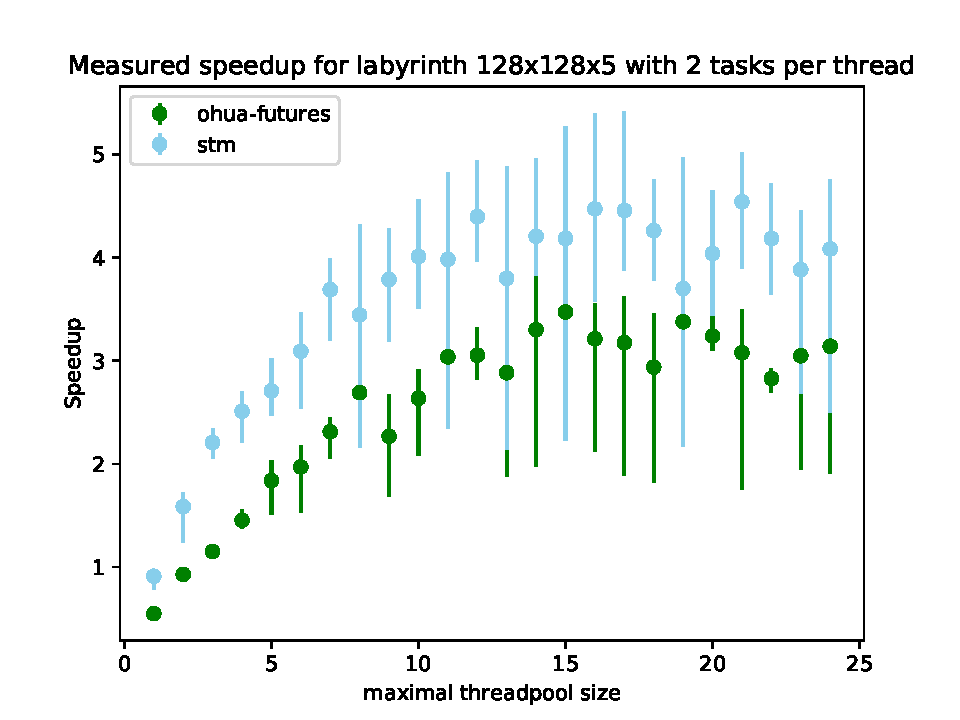
\includegraphics[width=.5\textwidth,keepaspectratio]{gfx/preliminaries-labyrinth/current-128x128x5}
    \caption{Measured speedup for an Ohua implementation using worklist splits, an update frequency of $2 \cdot threadcount$ and a work-stealing runtime.}%
    \label{fig:preliminaries:future-results}
\end{figure}



% - present our first look into the problem that was intended to show how fit or unfit Ohua was
% - explain that we looked into "labyrinth" and show our performance
% - detail the research we did on this and what our ideas were that we explored
%   - explain how we formulated 3 optimizations to tackle the problem but don't explain them all that general but more focused on the issue at hand
%   - show effect that the optimizations had
% - show end result which validated our assumption that this could work



















































